\section{Weight Agnostic Neural Networks}

\begin{figure}[h]
    \begin{center}
        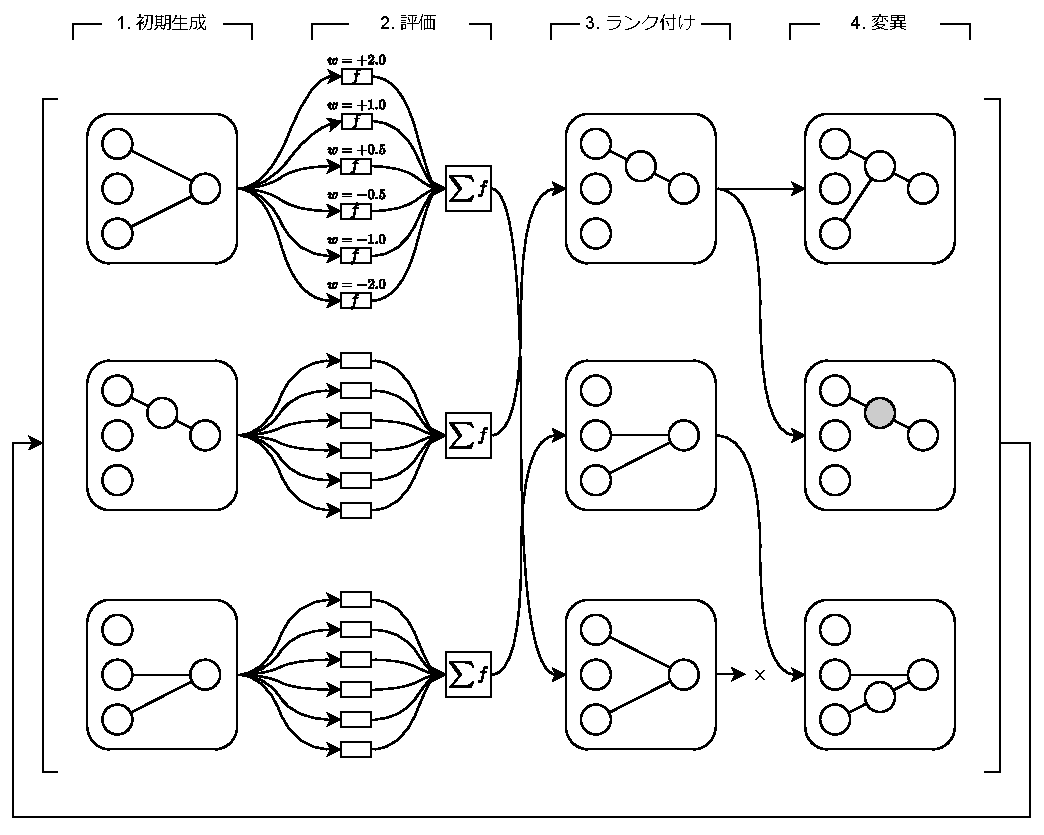
\includegraphics[scale=0.8]{img/expwann.pdf}
        \caption{WANNsの概略図}
    \end{center}
\end{figure}

Weight Agnostic Neural Networks(WANNs)は,2019年にAdam GaierとDavid Haによって発表されたニューラルネットワークの構造探索アルゴリズムである\cite{WANN}.WANNは,NEAT\cite{NEAT}をベースに作られており,これは遺伝的アルゴリズム\cite{遺伝的アルゴリズム}を用いたNeuro-Evolution\cite{NE}の手法から実現できる.多くのニューラルネットワークはシナプス荷重を更新することで,ネットワークの精度を向上させているが,WANNsによって生成された個体は,ネットワーク構造自体がタスクを解く性質を持っており,どんなシナプス荷重においてもそれなりの精度でタスクを解くことができる.これは生物の先天的能力と似た性質であると言える\cite{先天的能力}.また,WANNsネットワークはそれぞれのノードが別々の活性化関数を持っている.WANNの概略図を図3に示す.WANNにおける探索は以下の動作によって実現する.

\begin{enumerate}
    \item 初期生成
    個体は最初,最もシンプルな構造を持つネットワークからなる.中間層は存在せず,入力層のうちの一部からシナプスが出力層に接続されている.

    \item 評価
    各個体に対して,ネットワーク全体の共有重みを使用してタスクを実行する.本論文では, $ -2.0, -1.0, -0.5, +0.5, +1.0, +2.0 $ の6つの共有重みを使用する.また,タスクを解く際の初期状態により優れた結果を残せずに誤った評価をしないよう,それぞれの共有重みにて4回のタスクを実行する.最終的に6つの共有重みと4回の試行から得られた24個の評価値を合計する.

    \item ランク付け
    個体をランク付けする.上位の優れた個体は変更のないまま次世代へ保存され,下位の劣った個体は淘汰される.このランク付けはネットワークの評価値とネットワークの複雑さから算出される.

    \item 変異
    個体をランクのトーナメント選択\cite{遺伝的アルゴリズム}によって選択し,変異を起こした次世代の個体として保存する.

    保存された個体は再度評価,ランク付け,変異を行い,任意の世代数まで繰り返される.
\end{enumerate}

\subsection{変異}

\begin{figure}[h]
    \begin{center}
        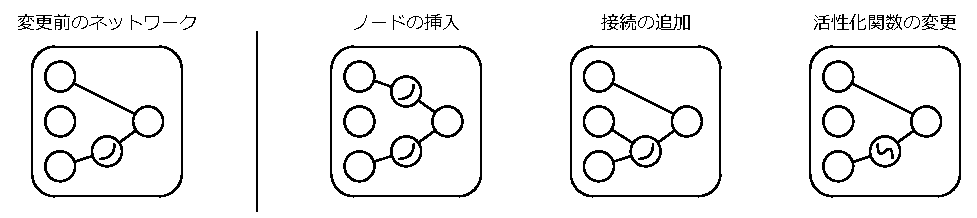
\includegraphics[scale=0.8]{img/vary.pdf}
        \caption{WANNsのネットワーク変異}
    \end{center}
\end{figure}

図に示したように,個体の変異にはノードの挿入,接続の追加,活性化関数の変更のいずれかを行い,各操作の具体的な手順は以下のようになる.

\begin{enumerate}
    \item ノードの挿入
    ネットワークの持つひとつの接続をランダムに選択し,接続の途中にひとつのノードを追加する.この時の活性化関数はランダムに選択される.

    \item 接続の追加
    接続を持たないふたつのノードを選択し,それらをつなぐ接続を追加する.

    \item 活性化関数の変更
    ネットワークの持つ中間層のノードを選択し,そのノードの活性化関数を変更する.活性化関数は現在選択されている関数以外の関数がランダムに選択される.このときの活性化関数はlinear, step, sin, cosine, Gaussian, tanh, sigmoid, inverse, absolute value, ReLUを利用する.
\end{enumerate}